\let\negmedspace\undefined
\let\negthickspace\undefined
\documentclass[journal]{IEEEtran}
\usepackage[a5paper, margin=10mm, onecolumn]{geometry}
%\usepackage{lmodern} % Ensure lmodern is loaded for pdflatex
\usepackage{tfrupee} % Include tfrupee package

\setlength{\headheight}{1cm} % Set the height of the header box
\setlength{\headsep}{0mm}     % Set the distance between the header box and the top of the text

\usepackage{gvv-book}
\usepackage{gvv}
\usepackage{cite}
\usepackage{amsmath,amssymb,amsfonts,amsthm}
\usepackage{algorithmic}
\usepackage{graphicx}
\usepackage{textcomp}
\usepackage{xcolor}
\usepackage{txfonts}
\usepackage{listings}
\usepackage{enumitem}
\usepackage{mathtools}
\usepackage{gensymb}
\usepackage{comment}
\usepackage[breaklinks=true]{hyperref}
\usepackage{tkz-euclide} 
\usepackage{listings}
% \usepackage{gvv}                                        
\def\inputGnumericTable{}                                 
\usepackage[latin1]{inputenc}                                
\usepackage{color}                                            
\usepackage{array}                                            
\usepackage{longtable}                                       
\usepackage{calc}                                             
\usepackage{multirow}                                         
\usepackage{hhline}                                           
\usepackage{ifthen}                                           
\usepackage{lscape}
\begin{document}

\bibliographystyle{IEEEtran}
\vspace{3cm}

\title{8.3.12}
\author{EE24BTECH11012 - Bhavanisankar G S}
% \maketitle
% \newpage
% \bigskip
{\let\newpage\relax\maketitle}

\renewcommand{\thefigure}{\theenumi}
\renewcommand{\thetable}{\theenumi}
\setlength{\intextsep}{10pt} % Space between text and floats


\numberwithin{equation}{enumi}
\numberwithin{figure}{enumi}
\renewcommand{\thetable}{\theenumi}

\textbf{QUESTION} : \\
Find the area bounded by the curves $\cbrak{\brak{x,y} : y \geq x^2  \text{ and } y = \abs{x} }$ \\
\textbf{SOLUTION} : \\
\textbf{Theoritical} : \\
\begin{enumerate}
	\item \textbf{FINDING THE POINT OF INTERSECTION} : \\
		General equation of a conic can be expressed as
		\begin{align}
			g(x) : \vec{x}^T\vec{v}\vec{x} + 2\vec{u}^T\vec{x} + f &= 0 \label{eq:conic}
		\end{align}
		The given curve can be expressed as a conic with formula
		\begin{align}
			\vec{V} &= \myvec{ 1 & 0 \\ 0 & 0 } \\
			\vec{u} &= \myvec{ 0 \\ \frac{-1}{2} } \\
			f &= 0
		\end{align}
		General equation of a line can be expressed as
		\begin{align}
			L : \vec{x} &= \vec{h} + k\vec{m} \label{eq:line}
		\end{align}
		The given line equation can be written as
		\begin{align}
			\vec{h} &= \myvec{0 \\ 0} \\
			\vec{m} &= \myvec{1 \\ 1}
		\end{align}
		Point of intersection of a line \eqref{eq:line} with a conic \eqref{eq:conic} is given by
		\begin{align}
			\vec{x}_{i} &= \vec{h} + k_{i} \vec{m} \label{eq:subs}
		\end{align}
		where, 
		\begin{align}
			k_i &= \frac{1}{\vec{m}^T\vec{v}\vec{m}} \brak{ -\vec{m}^T \brak{\vec{V}\vec{h} + \vec{u}} \pm \sqrt{ \brak{\vec{V}\vec{h} + \vec{u}}^2 - g(\vec{h}) \brak{\vec{m}^T\vec{v}\vec{m}}}} 
		\end{align}
		Substituting the given parameters in \eqref{eq:subs}, we have
		\begin{align}
			\vec{x}_1 &= \myvec{ 0 \\ 0 } \\
			\vec{x}_2 &= \myvec{ 1 \\ 1 } 
		\end{align}
	\item \textbf{EVALUATING THE INTEGRAL } : \\
	From the graph, it can be seen that 
	\begin{align}
		x \geq x^2 \text{ for } 0 \leq x \leq 1
	\end{align}
	Hence, the integral becomes
	\begin{align}
		A &= 2 \brak{ \int_{0}^{1} \brak{x - x^2} dx }\\
		A &= 2 \brak{ \left[ \frac{x^2}{2} - \frac{x^3}{3} \right]_{0}^{1} } \\
		A &= 2 \brak{ \frac{1}{2} - \frac{1}{3} }\\
		A &= 2 \brak{ \frac{1}{6} } \\
		A &= \frac{1}{3}
	\end{align}
	Hence, the area bounded by the given curves is $\frac{1}{3}$. \\
\end{enumerate}
\textbf{Simulation } : 
\begin{enumerate}
\item For a general interval, say $\sbrak{a,b}$, split up the intervals into $n$ parts such that
\begin{align}
	h &= \frac{b-a}{n} \label{eq:split}
\end{align}
\item Consider the points 
\begin{align}
	x_{0} &= a \\
	x_{n} &= b \\
	x_{i+1} &= x_{i} + h
\end{align}
\item \textbf{Trapezoid rule} : \\
Summing the areas of the trapezoids formed, we have
\begin{align}
	f(x) &= x - x^2 \\
	A &\approx \frac{h}{2} \brak{(f(x_{0}) + f(x_{1})) + (f(x_{1}) + f(x_{2})) + \dots + (f(x_{n-1}) + f(x_{n}))} \\
	A &\approx \frac{h}{2} \brak{f(x_{0}) + 2 \sum_{i=1}^{n-1} f(x_{i}) + f(x_{n}) } \label{eq:dif}
\end{align}
In the given question, 
\begin{align}
	a &= 0 \\
	b &= 1
\end{align}
Clearly, 
\begin{align}
	f(a) = f(b) = 0
\end{align}
since both the curves have $(0,0)$ and $(1,1)$ as their common points. Simplifying from \eqref{eq:split} and \eqref{eq:dif}, we have
\begin{align}
	A &\approx \frac{1}{n} \brak{\sum_{i=1}^{n-1} x_{i} - x_{i}^2 } \\
	A &\approx \frac{1}{n} \brak{\sum_{i=1}^{n-1} \frac{i}{n}  - (\frac{i}{n} )^2 } \\
	A &\approx \frac{1}{n^2} \brak{ \sum_{i=1}^{n-1} \brak{i - \frac{i^2}{n} } } \label{eq:diff}
\end{align}
Consider
\begin{align}
A_{n+1} &= A_{n} + \frac{h}{2} \brak{y_{n} + y_{n+1}} \\
A_{n+1} &= A_{n} + \frac{h}{2} \brak{y_{n} + \brak{y_{n} + h y^{\prime}_{n}}} \\
A_{n+1} &= A_{n} + \frac{h}{2} \brak{y_{n} + \brak{y_{n} + h (1 - 2x_{n} )} } \\
A_{n+1} &= A_{n} + \frac{h}{2} \brak{2 y_{n} + h \brak{1 - 2 x_{n}}}
\end{align}
which is the required difference equation.
\item The above equation can be coded to obtain the area bounded by the two curves.
\item It can be seen that the approximate solution turns out to be 0.3333333299999998.
\end{enumerate}
\begin{figure}[h]
\centering
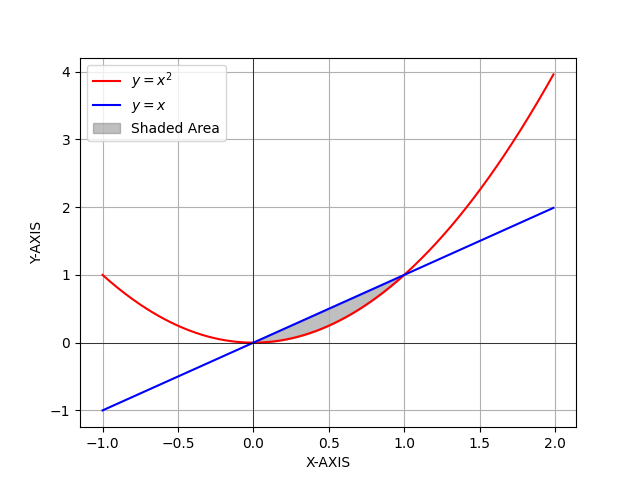
\includegraphics[width=\columnwidth]{figs/fig.png}
\caption{Plot of the given question.}
\label{fig:Plot1} 
\end{figure}
\end{document}
